% Options for packages loaded elsewhere
\PassOptionsToPackage{unicode}{hyperref}
\PassOptionsToPackage{hyphens}{url}
%
\documentclass[
]{article}
\usepackage{lmodern}
\usepackage{amssymb,amsmath}
\usepackage{ifxetex,ifluatex}
\ifnum 0\ifxetex 1\fi\ifluatex 1\fi=0 % if pdftex
  \usepackage[T1]{fontenc}
  \usepackage[utf8]{inputenc}
  \usepackage{textcomp} % provide euro and other symbols
\else % if luatex or xetex
  \usepackage{unicode-math}
  \defaultfontfeatures{Scale=MatchLowercase}
  \defaultfontfeatures[\rmfamily]{Ligatures=TeX,Scale=1}
\fi
% Use upquote if available, for straight quotes in verbatim environments
\IfFileExists{upquote.sty}{\usepackage{upquote}}{}
\IfFileExists{microtype.sty}{% use microtype if available
  \usepackage[]{microtype}
  \UseMicrotypeSet[protrusion]{basicmath} % disable protrusion for tt fonts
}{}
\makeatletter
\@ifundefined{KOMAClassName}{% if non-KOMA class
  \IfFileExists{parskip.sty}{%
    \usepackage{parskip}
  }{% else
    \setlength{\parindent}{0pt}
    \setlength{\parskip}{6pt plus 2pt minus 1pt}}
}{% if KOMA class
  \KOMAoptions{parskip=half}}
\makeatother
\usepackage{xcolor}
\IfFileExists{xurl.sty}{\usepackage{xurl}}{} % add URL line breaks if available
\IfFileExists{bookmark.sty}{\usepackage{bookmark}}{\usepackage{hyperref}}
\hypersetup{
  pdftitle={smartPARE degradome-seq analysis refinements},
  hidelinks,
  pdfcreator={LaTeX via pandoc}}
\urlstyle{same} % disable monospaced font for URLs
\usepackage[margin=1in]{geometry}
\usepackage{color}
\usepackage{fancyvrb}
\newcommand{\VerbBar}{|}
\newcommand{\VERB}{\Verb[commandchars=\\\{\}]}
\DefineVerbatimEnvironment{Highlighting}{Verbatim}{commandchars=\\\{\}}
% Add ',fontsize=\small' for more characters per line
\usepackage{framed}
\definecolor{shadecolor}{RGB}{248,248,248}
\newenvironment{Shaded}{\begin{snugshade}}{\end{snugshade}}
\newcommand{\AlertTok}[1]{\textcolor[rgb]{0.94,0.16,0.16}{#1}}
\newcommand{\AnnotationTok}[1]{\textcolor[rgb]{0.56,0.35,0.01}{\textbf{\textit{#1}}}}
\newcommand{\AttributeTok}[1]{\textcolor[rgb]{0.77,0.63,0.00}{#1}}
\newcommand{\BaseNTok}[1]{\textcolor[rgb]{0.00,0.00,0.81}{#1}}
\newcommand{\BuiltInTok}[1]{#1}
\newcommand{\CharTok}[1]{\textcolor[rgb]{0.31,0.60,0.02}{#1}}
\newcommand{\CommentTok}[1]{\textcolor[rgb]{0.56,0.35,0.01}{\textit{#1}}}
\newcommand{\CommentVarTok}[1]{\textcolor[rgb]{0.56,0.35,0.01}{\textbf{\textit{#1}}}}
\newcommand{\ConstantTok}[1]{\textcolor[rgb]{0.00,0.00,0.00}{#1}}
\newcommand{\ControlFlowTok}[1]{\textcolor[rgb]{0.13,0.29,0.53}{\textbf{#1}}}
\newcommand{\DataTypeTok}[1]{\textcolor[rgb]{0.13,0.29,0.53}{#1}}
\newcommand{\DecValTok}[1]{\textcolor[rgb]{0.00,0.00,0.81}{#1}}
\newcommand{\DocumentationTok}[1]{\textcolor[rgb]{0.56,0.35,0.01}{\textbf{\textit{#1}}}}
\newcommand{\ErrorTok}[1]{\textcolor[rgb]{0.64,0.00,0.00}{\textbf{#1}}}
\newcommand{\ExtensionTok}[1]{#1}
\newcommand{\FloatTok}[1]{\textcolor[rgb]{0.00,0.00,0.81}{#1}}
\newcommand{\FunctionTok}[1]{\textcolor[rgb]{0.00,0.00,0.00}{#1}}
\newcommand{\ImportTok}[1]{#1}
\newcommand{\InformationTok}[1]{\textcolor[rgb]{0.56,0.35,0.01}{\textbf{\textit{#1}}}}
\newcommand{\KeywordTok}[1]{\textcolor[rgb]{0.13,0.29,0.53}{\textbf{#1}}}
\newcommand{\NormalTok}[1]{#1}
\newcommand{\OperatorTok}[1]{\textcolor[rgb]{0.81,0.36,0.00}{\textbf{#1}}}
\newcommand{\OtherTok}[1]{\textcolor[rgb]{0.56,0.35,0.01}{#1}}
\newcommand{\PreprocessorTok}[1]{\textcolor[rgb]{0.56,0.35,0.01}{\textit{#1}}}
\newcommand{\RegionMarkerTok}[1]{#1}
\newcommand{\SpecialCharTok}[1]{\textcolor[rgb]{0.00,0.00,0.00}{#1}}
\newcommand{\SpecialStringTok}[1]{\textcolor[rgb]{0.31,0.60,0.02}{#1}}
\newcommand{\StringTok}[1]{\textcolor[rgb]{0.31,0.60,0.02}{#1}}
\newcommand{\VariableTok}[1]{\textcolor[rgb]{0.00,0.00,0.00}{#1}}
\newcommand{\VerbatimStringTok}[1]{\textcolor[rgb]{0.31,0.60,0.02}{#1}}
\newcommand{\WarningTok}[1]{\textcolor[rgb]{0.56,0.35,0.01}{\textbf{\textit{#1}}}}
\usepackage{longtable,booktabs}
% Correct order of tables after \paragraph or \subparagraph
\usepackage{etoolbox}
\makeatletter
\patchcmd\longtable{\par}{\if@noskipsec\mbox{}\fi\par}{}{}
\makeatother
% Allow footnotes in longtable head/foot
\IfFileExists{footnotehyper.sty}{\usepackage{footnotehyper}}{\usepackage{footnote}}
\makesavenoteenv{longtable}
\usepackage{graphicx,grffile}
\makeatletter
\def\maxwidth{\ifdim\Gin@nat@width>\linewidth\linewidth\else\Gin@nat@width\fi}
\def\maxheight{\ifdim\Gin@nat@height>\textheight\textheight\else\Gin@nat@height\fi}
\makeatother
% Scale images if necessary, so that they will not overflow the page
% margins by default, and it is still possible to overwrite the defaults
% using explicit options in \includegraphics[width, height, ...]{}
\setkeys{Gin}{width=\maxwidth,height=\maxheight,keepaspectratio}
% Set default figure placement to htbp
\makeatletter
\def\fps@figure{htbp}
\makeatother
\setlength{\emergencystretch}{3em} % prevent overfull lines
\providecommand{\tightlist}{%
  \setlength{\itemsep}{0pt}\setlength{\parskip}{0pt}}
\setcounter{secnumdepth}{-\maxdimen} % remove section numbering

\title{smartPARE degradome-seq analysis refinements}
\author{}
\date{\vspace{-2.5em}}

\begin{document}
\maketitle

\textbf{smartPARE} is an R package designed for sRNA cleavage
confirmation based on degradome data. smartPARE utilizes deep sequencing
convolutional neural networks (CNN) to segregate true and false
predictions of sRNA cleavage data produced by any sRNA cleavage
prediction tool.

\textbf{Overview} - smartPARE consists of the 3 following stages:

\begin{enumerate}
\def\labelenumi{\arabic{enumi}.}
\tightlist
\item
  Generation of cleavage windows
\item
  Cleavage window training
\item
  Cleavage confirmations
\end{enumerate}

\begin{center}\rule{0.5\linewidth}{0.5pt}\end{center}

\hypertarget{installation}{%
\section{Installation}\label{installation}}

\begin{Shaded}
\begin{Highlighting}[]
\CommentTok{#Installation requires devtools}
\CommentTok{#install.packages("devtools")}
\NormalTok{devtools}\OperatorTok{::}\KeywordTok{install_github}\NormalTok{(}\StringTok{'kristianHoden/smartPARE'}\NormalTok{)}
\CommentTok{#Load the smartPARE R package}
\KeywordTok{library}\NormalTok{(smartPARE)}
\end{Highlighting}
\end{Shaded}

\begin{center}\rule{0.5\linewidth}{0.5pt}\end{center}

\hypertarget{generation-of-cleavage-windows}{%
\section{Generation of cleavage
windows}\label{generation-of-cleavage-windows}}

smartPARE identifies cleavages based on images of the sRNA cleavages
sites (windows). The windows are created from degradome sequencing data
transcript-aligned bam-files. The standard length of dagradome-seq reads
are 20 nt. Hence, the default windows are generated from an area 1
nucleotides (nt) upstream the cleavage site to 21 nt downstream. The
narrow mariginal to the proposed cleavage site reads to exclude as much
noise as possible but still include the characteristic cleavage block
(seen in the following image).\\
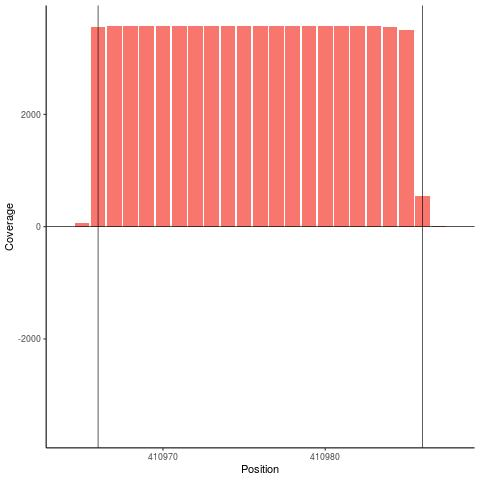
\includegraphics{images/cleavage.jpg}

\begin{verbatim}
smartPARE_cleavageWindows(dirO = "pathOut/dir_smart"),
cleavageData = cleavageDataDataset,
aliFilesPath = "path/bamTranscriptome/",
aliFilesPattern1 = "pattern1.sorted.bam$",
aliFilesPattern2 = "pattern2.sorted.bam$",
ylim1 = 5,
edgesExtend1 = c(1,21),
gffTrans = gffTrans)
\end{verbatim}

\textbf{Parameters:}

\texttt{gffTrans} - a dataframe of your imported gff with V10 =
transcript ID. See for example extendGffTrans for example

\texttt{aliFilesPattern1} - regular expression defining the pattern of
the first degradome bam file

\texttt{aliFilesPattern2} - regular expression defining the pattern of
the second bam file

\texttt{dirO} - output path. Please end the path with \_extension to
make the dirs identifiable by smartPARE.

\texttt{cleavageData} - a dataframe containing at least columns genesT
(the target genes) and posT (target position in the transcript)

\texttt{edgesExtend1} - Nt positions in relation to the cleavage site
that are included in the images. Witten in the format:
\texttt{c(upstream,downstream)}. Default is c(1,21).

\texttt{ylim1} - The minimum plotted height on the y-axis. In practise
this means that a lower ``cleavage block'' might not be recognized by
the CNN. This to exclude potential false positives caused by noice.

\texttt{aliFilesPath} - path to the bam files of the user defined
degradome.

\textbf{Output:}

Images displaying in the output dir \texttt{dirO} the read coverage
surrounding the cleavage site labeled
\texttt{transcriptID\_cleavagePosition}

\begin{center}\rule{0.5\linewidth}{0.5pt}\end{center}

\hypertarget{cleavage-window-training}{%
\section{Cleavage window training}\label{cleavage-window-training}}

This stage is only necessary if deciding to create a new CNN model. Our
pre-trained model is found in
\href{../data/model/CNNmodel.h5}{../data/model/}

\textbf{Preparation:}

\begin{itemize}
\tightlist
\item
  Create a directory called train with three subdirs called goodUp,
  goodDown and bad.
\item
  Collect manually identified images of true cleavages on the 5' strand
  in the goodUp subdir.
\item
  Collect manually identified images of true cleavages on the 3' strand
  in the goodDown subdir.
\item
  Collect manually identified images of false cleavages in the the bad
  subdir.
\item
  \textbf{N.B.} Ensure to get as great variation as possible among the
  images of each subdir.\\
\end{itemize}

\begin{verbatim}
modelData <- smartPARE_train(homePath1 = "example/",
                             pixels1 = 28,
                             search_bound = list(denseLoop = c(0,4),  
                                                 epochs2 = c(100, 300),  
                                                 batch_size2 = c(32,128),  
                                                 dropout2 = c(0, 0.3),  
                                                 validation_split2 = c(0.1,0.4),  
                                                 convolutionalLoop = c(1,4),  
                                                 NO_pooling2 = c(1,2)),
                             n_iter = 100)
\end{verbatim}

\textbf{Parameters:}

\texttt{homePath1} Path to the root directory of the train directory
metioned above.

\texttt{pixels1} Number of pixels each each image will be converted to
\texttt{search\_bound} List of min and max values for the following
variables: denseLoop2, epochs2, batch\_size2, validation\_split2,
convolutionalLoop2 and NO\_pooling2

\texttt{n\_iter} Number of iterations the Bayesian optimization will
run, each run creating a model

\textbf{Output:}

\texttt{modelData} contains a list with the following 4 entries:

\begin{enumerate}
\def\labelenumi{\arabic{enumi}.}
\item
  \texttt{\$Best\_Par} shows the hyperparameters for the best performing
  model.
\item
  \texttt{\$Best\_Value} displays the score of the best model. The score
  is based on the inverted loss of the model.
\item
  \texttt{\$History} the history of hyperparameters for all the created
  models.
\item
  \texttt{\$Pred} the inverted loss of the cross-validated data.
\end{enumerate}

Each created model is witten into ``homePath1/bayesmodels/'', where a
subdir (``pdf'') with pdfs displaying the performance of each model also
is found. The model names in the directory is based on the iteration
order followed by then accuracy (0-1), then loss, then the value of each
hyperparameter. This makes it possible to identify the performance and
setting of the model even if the \texttt{modelData} info is lost.

\begin{center}\rule{0.5\linewidth}{0.5pt}\end{center}

\hypertarget{cleavage-confirmations}{%
\section{Cleavage confirmations}\label{cleavage-confirmations}}

\textbf{Preparation} Gather images that you want to evaluate in subdirs
to your wd (homePath1) at a certain level of recursion. Please end the
dirs with \_extension e.g.~example\_smart. The underline will be
identified by smartPARE indicate that these dirs contains cleavage
images. In an interaction study you might for example have cleavages
from 2 different species gathered in different subdirs (specie1 \&
specie2). Maybe you also have different timepoints for each specie (tp1
\& tp2). You might then gather your images in homePath1/specie1/tp1/
etc. The level of recursion will then be 3.

Load the preferred model according to one of the following:

If you designed your own model

\texttt{model\ \textless{}-\ keras::load\_model\_hdf5("example/bayesmodels/modelNumberAndContinousName.h5")}

If you are using our model\\
\texttt{model\ \textless{}-\ keras::load\_model\_hdf5("data/model/CNNmodel.h5")}

View the loaded model

\begin{verbatim}
`model %>% summary()` 
\end{verbatim}

Define the directories you want to examine\\
\texttt{extDirs\ \textless{}-\ unique(dirname(list.files(homePath1,rec=T)))}

Exclude the training dirs (if they are in the same path)

\begin{verbatim}
extDirs[-which(startsWith(prefix = "train",extDirs))]  
extDirs <- extDirs[-which(startsWith(prefix = "train",extDirs))]  
rootExt <- paste0(homePath1,extDirs)
\end{verbatim}

Examine the cleavages images in rootExt dirs. \texttt{pixels} must be
the same as when creating the model. Our model was based on 28 pixels.

\begin{verbatim}
smartPARE_examineCleavages(examinePath = rootExt, model = model,pixels = 28) 
\end{verbatim}

Construct a list of the true cleavages, \texttt{recursionLevel} counts
the homePath1 level as level 0. the first subdir level is level 1 etc.
Example images are found in `example/evaluate\_smart/".

\begin{verbatim}
smartPARE_ListTrue(pathToTrue = homePath1,recursionLevel = 0)  
\end{verbatim}

\textbf{Output}

Output will be written to your homePath into a dir called
``subdir''\_results, e.g.~example\_results

Extract the information about the true cleavage windows from your
results file

\begin{verbatim}
trueCleavagesDf <- smartPARE_parse(smartPAREresultFile = paste0(homePath1,"example_results/true.txt"))
\end{verbatim}

\textbf{Output}

\texttt{trueCleavagesDf} contains the following four columns that can be
used to filter out false cleavage sites in the dataset used for
generating the cleavage images:

\begin{itemize}
\tightlist
\item
  ds, (dataset) based on the name of the dir the cleavage images were
  stored in
\item
  posT, cleavage position in the transcript
\item
  ext, the extension of the cleavage images\\
\item
  transcript, transcript ID
\end{itemize}

\begin{longtable}[]{@{}lrll@{}}
\toprule
ds & posT & ext & transcript\tabularnewline
\midrule
\endhead
evaluate & 987 & R1.jpg & PGSC0003DMG400002426\tabularnewline
evaluate & 987 & R2.jpg & PGSC0003DMG400002426\tabularnewline
evaluate & 988 & R1.jpg & PGSC0003DMG400002426\tabularnewline
evaluate & 1072 & R2.jpg & PGSC0003DMT400006358\tabularnewline
evaluate & 1363 & R2.jpg & PGSC0003DMT400006361\tabularnewline
\bottomrule
\end{longtable}

\end{document}
